\section{Exploratory analysis}
\label{sec:eda}

\subsection{Quantitative variables}

\subsubsection{Quartiles and outlier bounds}

The quartiles and $1.5\times$IQR bounds of the hourly variables are reported
in their original units (\cref{tab:cuartiles-iqr}) and are the same ones the
cleaning used as the outlier criterion. \texttt{RAINF} and \texttt{WDR} are
excluded: \texttt{WDR} is circular and \texttt{RAINF} is zero-inflated, so
their IQR cannot be interpreted as a bound (\cref{sec:dic:meteorologicos}).
Two readings matter for what follows: the median zonal wind component is
negative, that is, the prevailing wind enters from the east
(\cref{sec:contexto-estaciones}); and the upper bound of \texttt{O3\_8h}
(66.22 ppb) lies above the 51 ppb threshold, so exceedance is not an outlier
but part of the usual range of the variable.

\begin{table}[t]
  \centering
  \caption{Quartiles and outlier bounds ($1.5\times$IQR criterion) of the
    hourly quantitative variables, in their original units.}
  \label{tab:cuartiles-iqr}
  \small
  \begin{tabular}{lrrrr}
    \toprule
    Variable & Q1 & Q3 & Lower & Upper \\
    \midrule
    \texttt{O3}       &    13.00 &    37.00 &  $-23.00$ &    73.00 \\
    \texttt{CO}       &     0.71 &     1.83 &   $-0.96$ &     3.50 \\
    \texttt{NO2}      &     6.90 &    19.70 &  $-12.30$ &    38.90 \\
    \texttt{NOX}      &    10.95 &    30.70 &  $-18.68$ &    60.33 \\
    \texttt{PM10}     &    35.00 &    74.00 &  $-23.50$ &   132.50 \\
    \texttt{PM2.5}    &    10.00 &    26.74 &  $-15.11$ &    51.85 \\
    \texttt{TOUT}     &    18.49 &    28.39 &      3.64 &    43.24 \\
    \texttt{PRS}      &   709.70 &   721.70 &    691.70 &   739.70 \\
    \texttt{WSR}      &     4.70 &    11.60 &   $-5.65$ &    21.95 \\
    \texttt{O3\_8h}   &    15.44 &    35.75 &  $-15.03$ &    66.22 \\
    \texttt{viento\_u}&  $-8.56$ &     0.21 &  $-21.73$ &    13.37 \\
    \texttt{viento\_v}&  $-3.38$ &     3.98 &  $-14.41$ &    15.01 \\
    \bottomrule
  \end{tabular}
\end{table}

\Cref{fig:boxplot-medidas} shows the distribution of each variable in
original units. All pollutant concentrations have a long right tail, with
outliers several times the third quartile; this is the asymmetry that
motivated Box-Cox in \cref{sec:transformaciones}. The meteorological
variables are more symmetric, except wind speed.

\begin{figure}[t]
    \centering
    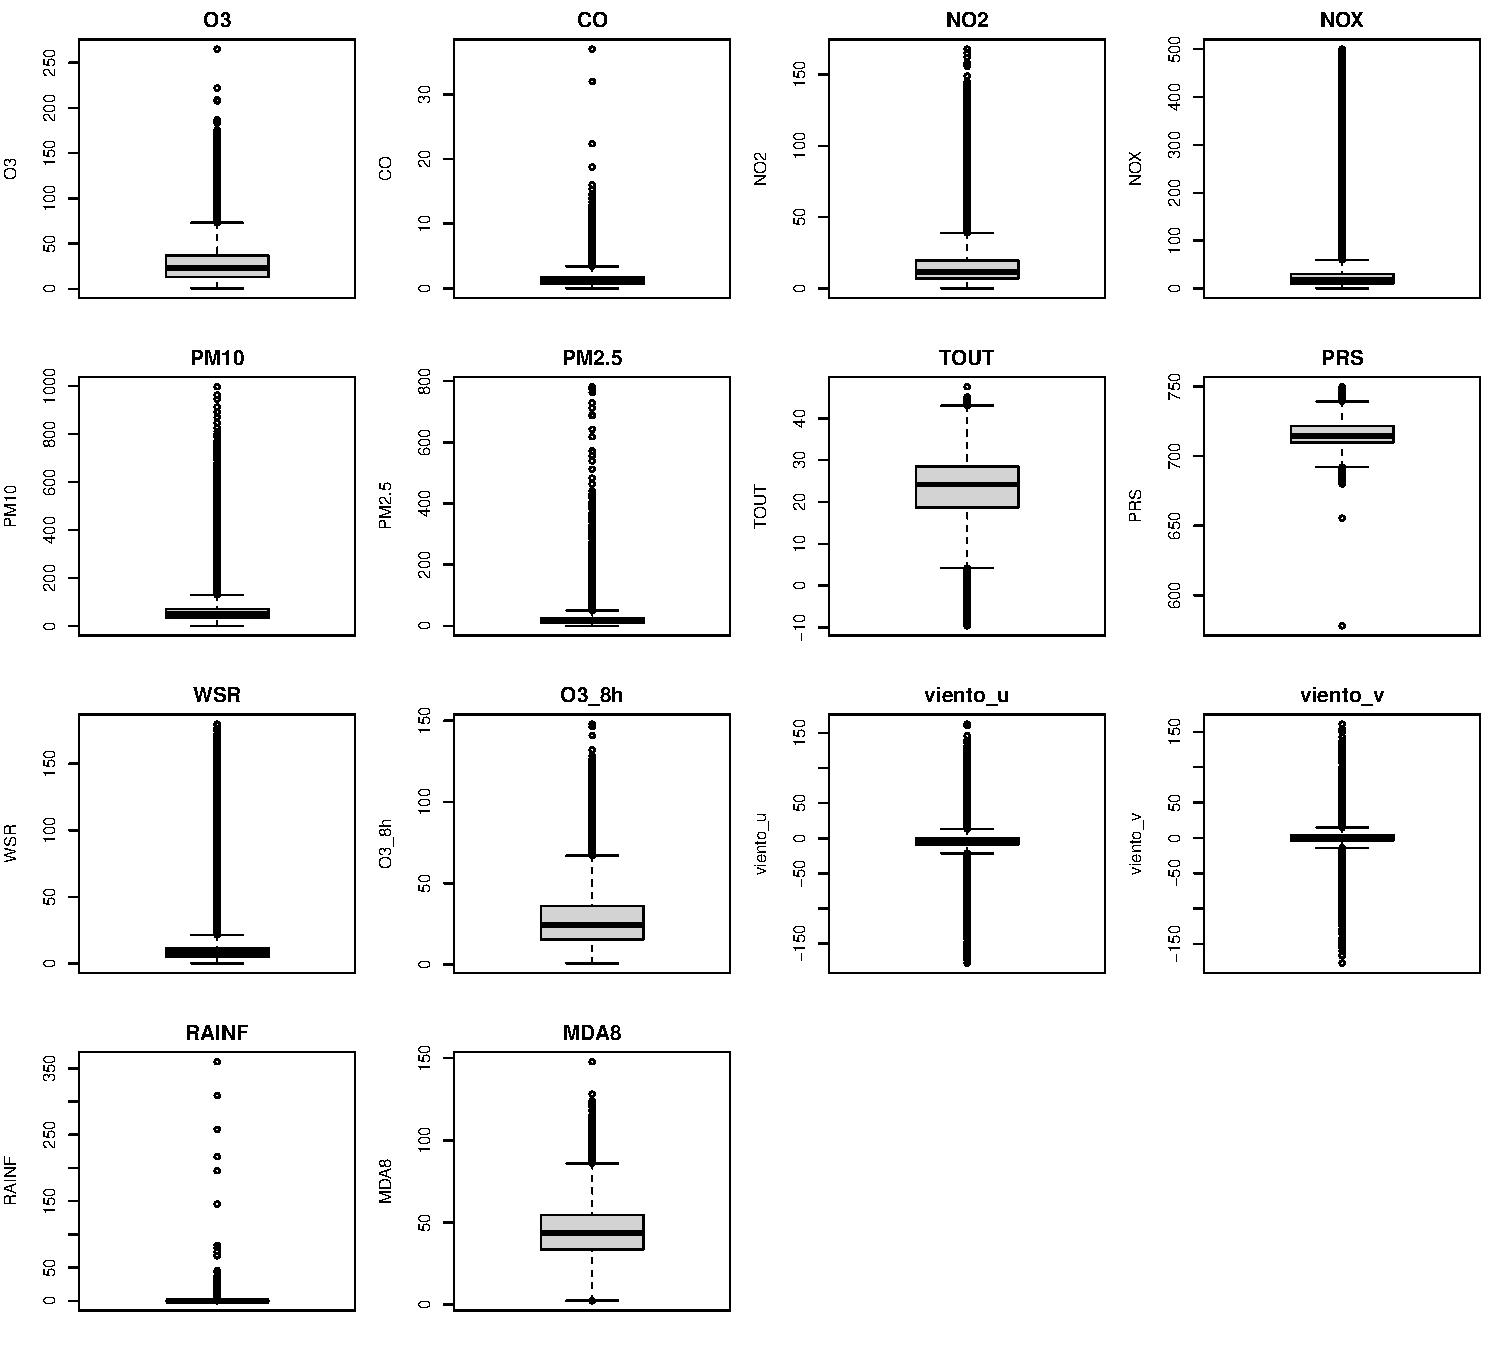
\includegraphics[width = \linewidth]{boxplots_medidas.pdf}
    \caption{Box plots of each hourly quantitative variable, in original
      units.}
    \label{fig:boxplot-medidas}
\end{figure}

\subsubsection{Correlation}

At hourly resolution and on the transformed scale, the strongest pairs are
\texttt{NO2}--\texttt{NOX} ($r=0.89$), the expected multicollinearity between
precursors of the same reaction cycle; \texttt{O3}--\texttt{O3\_8h}
($r=0.69$), by construction; \texttt{PM10}--\texttt{PM2.5} ($r=0.62$),
particulate matter of common origin; \texttt{O3}--\texttt{TOUT} ($r=0.52$)
and \texttt{O3}--\texttt{WSR} ($r=0.43$), consistent with the photochemical
mechanism; and \texttt{O3}--\texttt{NOX} ($r=-0.43$), which reflects the
consumption of \ce{O3} by titration with \ce{NO} near traffic sources.

PCA runs on the daily table and requires its own matrix: aggregating to days
changes the sample size and typically increases correlations by cancelling
measurement noise. It is computed over the 16 continuous variables of the
transformed daily dataset, on the subset with all 16 simultaneously complete
($n=15{,}856$ of 26,691 station-days, 59.4\,\%), the same listwise deletion
rule used in modeling, which guarantees a positive semidefinite matrix
(\cref{fig:mapa-calor-diario}).

\begin{figure}[t]
    \centering
    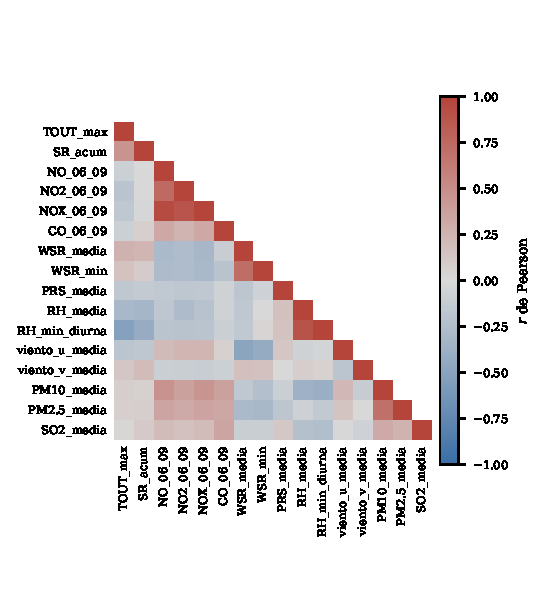
\includegraphics[width = \linewidth]{mapa_calor_correlacion_diario.pdf}
    \caption{Pearson correlation heat map of the 16 continuous variables of
      the transformed daily dataset, $n=15{,}856$ complete station-days.}
    \label{fig:mapa-calor-diario}
\end{figure}

Three hourly pairs have a direct analogue in the daily dataset:
\texttt{NO2}--\texttt{NOX} is unchanged (0.89), \texttt{PM10}--\texttt{PM2.5}
rises to 0.70, and \texttt{viento\_u}--\texttt{WSR} increases in magnitude to
$-0.48$. The ordering does change: \texttt{NO}--\texttt{NOX} ($r=0.95$) and
\texttt{RH\_media}--\texttt{RH\_min\_diurna} ($r=0.89$) dominate, absent from
the hourly map because \texttt{NO} and \texttt{RH} were not part of that set.
The first is the definitional redundancy \texttt{NOX} $\approx$ \texttt{NO} +
\texttt{NO2}; the second, and also \texttt{WSR\_media}--\texttt{WSR\_min}
($r=0.71$), is the same variable summarized twice over different windows of
the day. These construction redundancies are the ones that factor analysis
(\cref{sec:analisis-factorial}) eventually removes.

The diagnostics prior to PCA confirm the multicollinearity
(\cref{tab:diagnostico-pca}): the determinant is close to 0 and the condition
number is high. Bartlett's test of sphericity rejects that the matrix is the
identity ($\chi^2(120)=169{,}140.7$, $p<0.001$), and the overall KMO clears
the conventional threshold of 0.6; at the variable level, \texttt{RH\_media}
(0.587), \texttt{PRS\_media} (0.589) and \texttt{TOUT\_max} (0.596) fall just
below it without pulling down the total. The four diagnostics justify
applying PCA to the daily predictors.

\begin{table}[t]
  \centering
  \caption{Diagnostics prior to PCA on the daily correlation matrix
    ($n=15{,}856$, 16 variables).}
  \label{tab:diagnostico-pca}
  \small
  \begin{tabular}{lr}
    \toprule
    Diagnostic          & Value \\
    \midrule
    Determinant         & $2.32\times10^{-5}$ \\
    Condition number    & 322.8 \\
    Overall KMO         & 0.660 \\
    \bottomrule
  \end{tabular}
\end{table}
